\section{Introducción a IA}

La Inteligencia Artificial (IA) es como el hijo prodigio de la ciencia moderna, 
nacido poco después de la Segunda Guerra Mundial y oficialmente bautizado con su 
nombre en 1956. Desde entonces, ha pasado de ser una idea fascinante a un componente 
integral de nuestras vidas. ¿Quién no ha interactuado con un asistente virtual, 
o se ha maravillado con la habilidad de un programa para jugar al ajedrez? \\

Hoy en día, la IA es omnipresente, desde recomendaciones personalizadas en nuestras 
redes sociales hasta sistemas de navegación que nos guían por las calles. Es como 
el ingrediente secreto en la receta del progreso tecnológico, impulsando avances 
en medicina, transporte, finanzas y más. \\

Pero lo emocionante de la IA es que apenas estamos empezando a arañar la superficie 
de lo que es posible. Imagina un futuro donde los autos se conducen solos de manera 
más segura que los conductores humanos, donde los diagnósticos médicos son 
más precisos y rápidos, y donde la creatividad humana se ve amplificada 
por algoritmos inteligentes.


\subsection{Qué es la IA?}

Hemos dicho de donde viene, donde esta presente y a donde quiere ir la IA, pero cual 
es la definición. A lo largo de su historia, han surgido cuatro enfoques principales. 
Por un lado, están los enfoques centrados en los humanos, que ven a la IA como una 
ciencia empírica, con hipótesis que se prueban mediante experimentación. Por otro 
lado, están los enfoques centrados en la racionalidad, que implican una combinación 
de matemáticas e ingeniería. Estos dos enfoques a menudo entran en conflicto, 
pero también se han complementado mutuamente en el desarrollo de la IA.


\begin{center}
    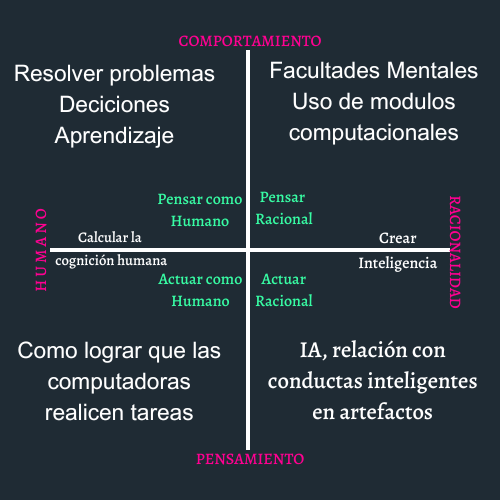
\includegraphics[scale = .8]{assets/imagenes/NT01.png}
\end{center}

\begin{myitemize}
    \item Sistemas que piensan como humanos
    
    Los chatbots de atención al cliente son un buen ejemplo. Utilizan algoritmos 
    de procesamiento de lenguaje natural para entender las preguntas y responder 
    de manera coherente, imitando el proceso de pensamiento humano en la conversación.

    \item Sistemas que actúan como humanos
    
    Los robots con capacidad de movimientos humanos, como Atlas de Boston Dynamics, 
    muestran esta característica. Atlas puede realizar una variedad de movimientos 
    físicos, desde caminar y correr hasta levantar objetos, todo imitando la forma 
    en que lo haría una persona. \cite{rtatlas}

    \item Sistemas que piensan racionalmente
    
    Los motores de recomendación de películas o música son ejemplos de sistemas que 
    utilizan la lógica y el razonamiento para generar recomendaciones personalizadas. 
    Estos sistemas analizan el historial de preferencias del usuario y aplican 
    algoritmos de aprendizaje automático para predecir qué contenido le gustaría 
    basado en patrones previos.
    

    \item Sistemas que actúan racionalmente
    
    Los vehículos autónomos son un ejemplo claro. Estos sistemas utilizan sensores, 
    cámaras y algoritmos avanzados para percibir su entorno, tomar decisiones en 
    tiempo real y navegar de manera segura por el tráfico, siguiendo las normas de 
    conducción y evitando obstáculos.
\end{myitemize}


Entonces una definición final sería:\\

\textit{La Inteligencia Artificial es el campo de estudio que se enfoca en 
desarrollar sistemas y tecnologías que pueden simular y/o mejorar la capacidad 
humana de pensar, razonar, actuar y aprender, ya sea imitando el pensamiento 
y comportamiento humano o aplicando procesos lógicos y racionales adaptándose 
a su entorno para resolver problemas y tomar decisiones en diversas 
áreas de aplicación}

\subsection*{Áreas de la IA}

\begin{myitemize}
    \item Procesamiento de Lenguaje Natural (NLP): Campo que se centra en la interacción 
    entre las computadoras y el lenguaje humano, permitiendo a las máquinas comprender, 
    interpretar y generar lenguaje humano.
    
    \item Visión por Computadora: Se refiere al desarrollo de sistemas que pueden 
    interpretar, analizar y comprender imágenes y videos digitales, imitando la 
    capacidad del sistema visual humano.

    \item Aprendizaje Automático (Machine Learning): Área de la IA que se enfoca 
    en el desarrollo de algoritmos y modelos que permiten a las computadoras 
    aprender de datos y realizar tareas específicas sin ser programadas explícitamente.
    
    \item Robótica: Combinación de hardware y software que permite diseñar, 
    construir y operar robots capaces de realizar diversas tareas de manera autónoma 
    o controlada por humanos.
    
    \item Reconocimiento de Voz: Tecnología que permite a las máquinas interpretar 
    y comprender el habla humana, convirtiendo el lenguaje hablado en texto o 
    comandos ejecutables.
    
    \item Inteligencia Artificial Explicable (XAI): Área que se centra en el 
    desarrollo de modelos y sistemas de IA que pueden explicar y justificar sus 
    decisiones y procesos de razonamiento de manera comprensible para los humanos.
    
    \item Sistemas de Recomendación: Tecnología utilizada para predecir y recomendar 
    productos, servicios o contenido personalizado a los usuarios, basándose en 
    sus preferencias y comportamientos anteriores.
    
    \item Procesamiento de Datos Masivos (Big Data): Conjunto de técnicas y 
    herramientas utilizadas para analizar, procesar y extraer información 
    significativa de conjuntos de datos extremadamente grandes y complejos.
    
    \item Automatización Robótica de Procesos (RPA): Tecnología que permite 
    automatizar tareas repetitivas y basadas en reglas dentro de procesos 
    empresariales, utilizando software para imitar la interacción humana 
    con sistemas digitales.
    
    \item Diagnóstico Médico Asistido por Computadora: Aplicación de la IA en el 
    campo de la medicina para ayudar en el diagnóstico y tratamiento de 
    enfermedades, mediante el análisis de datos médicos y la generación de 
    recomendaciones clínicas.
    
    \item Sistemas Autónomos: Sistemas o dispositivos que pueden operar de manera 
    independiente y autónoma sin intervención humana directa, tomando 
    decisiones y realizando acciones en función de su entorno y objetivos programados.
    
    \item Traducción Automática: Tecnología que permite la traducción automática 
    de texto o voz de un idioma a otro, utilizando modelos de IA entrenados en 
    datos lingüísticos multilingües.
    
    \item Realidad Aumentada (AR): Tecnología que combina elementos virtuales 
    generados por computadora con el entorno físico del usuario en tiempo real, 
    mejorando la experiencia perceptual y proporcionando información adicional.
    
    \item Predicción de Mercados Financieros: Aplicación de técnicas de IA para analizar 
    datos financieros y de mercado, con el objetivo de predecir tendencias, 
    fluctuaciones y comportamientos futuros en los mercados financieros.
    
    \item Bioinformática: Campo interdisciplinario que aplica técnicas de IA y 
    análisis de datos para estudiar y comprender fenómenos biológicos, como 
    la secuenciación del ADN, la modelización de proteínas y la predicción de 
    interacciones moleculares.
\end{myitemize}


\subsection{Tipos de aprendizaje}

\noindent \textcolor{Contraste4}{Aprendizaje Automático}\\

Este tipo de aprendizaje se trata de enseñar a las computadoras a aprender de los datos 
y tomar decisiones basadas en esos datos sin necesidad de programación explícita. En 
lugar de decirle a la máquina qué hacer paso a paso, le proporcionamos ejemplos y la 
dejamos descubrir patrones por sí misma. Por ejemplo, los algoritmos de aprendizaje 
automático pueden predecir si un correo electrónico es spam o no basándose en 
ejemplos anteriores\\


\noindent \textcolor{Contraste4}{Análisis del Tiempo}\\

Aquí nos centramos en entender y predecir patrones y tendencias en datos que varían 
con el tiempo. Desde prever la demanda de productos en una tienda hasta pronosticar 
el clima, el análisis del tiempo implica analizar datos cronológicos para entender 
cómo cambian las cosas con el tiempo y qué podemos esperar en el futuro.\\


\noindent \textcolor{Contraste4}{Análisis por Casos}\\

Este tipo de análisis se enfoca en resolver problemas basándose en la similitud con 
casos anteriores. Imagina que tienes un sistema que puede diagnosticar enfermedades 
basándose en síntomas similares a los de casos anteriores que ya ha visto. Eso es 
el análisis por casos: aprender de la experiencia pasada para resolver 
problemas en el futuro.\\ 


\noindent \textcolor{Contraste4}{Aprendizaje Supervisado}\\

Este es uno de los enfoques más comunes en el aprendizaje automático. Aquí, la máquina 
aprende a partir de ejemplos etiquetados, es decir, datos para los que ya conocemos 
las respuestas correctas. Por ejemplo, si queremos enseñar a una máquina a reconocer 
gatos en imágenes, le mostramos muchas imágenes de gatos etiquetadas como gato y 
muchas otras de cosas que no son gatos, etiquetadas como no gato. La máquina aprende 
a distinguir entre las dos categorías basándose en estos ejemplos.